\chapter{Designing Dynamic Mechanisms}
The realistic simulation of highly-dynamic elastic objects is important for a broad range of applications in computer graphics, engineering and computational fabrication. However, whether simulating flipping toys, jumping robots, prosthetics or quickly moving creatures, performing such simulations in the presence of contact, impact and friction is both time consuming and inaccurate. In this paper we present Dynamics-Aware Coarsening (DAC) and the Boundary Balanced Impact (BBI) model  which allow for the accurate simulation of dynamic, elastic objects undergoing both large scale deformation and frictional contact, at rates up to 79 times faster than state-of-the-art methods. DAC and BBI produce simulations that are accurate and fast enough to be used  (for the first time) for the computational design of 3D-printable compliant dynamic mechanisms. Thus we demonstrate the efficacy of DAC and BBI by designing and fabricating mechanisms which flip, throw and jump over and onto obstacles as requested.
\section{Introduction}

We present a pair of new methods to accurately simulate geometric and material nonlinearities subject to frictional contact, large loads and high-speed collisions at rates significantly more than an order-of-magnitude faster than previously available.
Our methods combine efficiency and accuracy to enable design-for-fabrication optimization. They can be used for both fast, realistic animation and engineering analysis. 

Here we look towards a new generation of efficient mechanisms for practical \emph{dynamic} function~\citep{Lipson:2014fa,Rus:2015eq,Reis:2015hb,Reis:2015ey}. In order to extend physics-driven computational design to this domain, however, a bottleneck must be overcome - the physical simulation itself. Simulations must accurately replicate the behavior of elastic materials subject to high-speed, transient dynamics. Modeling these systems combines many of the remaining grand challenges in simulating elastica. Specifically we must accurately resolve nonlinear elasticity, large deformations, stiff materials, high-speed dynamics, rapid loading and unloading, frictional contact, internal friction, high-speed collisions, and rebound. 

State-of-the-art FEM systems currently able to accurately match these effects are exceedingly expensive - runtimes on the order of days are standard to perform a single simulation in many cases~\citep{Belytschko:2013tz}. 
Thus, while generating a single simulation for visualization or animation is already time consuming, the many simulations required during design optimization compound an already prohibitive computational burden.
\subsection{Efficiency with Accuracy}
Let us explore four potential solutions for constructing fast \emph{and} accurate simulation algorithms: (1) higher-order elements, (2) adaptive meshes, (3) reduced models, and (4) numerical coarsening. Can these methods provide the necessary efficiency to enable design-optimization while obtaining the predictive accuracy required to match fabricated results?

\emph{Higher-order elements} offer us the opportunity to replace thin regions of our models with elements that capture higher-order deformation modes. While an attractive strategy, this poses two challenges. 
First, due to changing design parameters, we will need to identify suitable regions on-the-fly in order to perform this replacement. 
Second, coupling swapped-in higher-order elements to other element types introduces overhead. Consider, for example, replacing lower-order hexahedra with plate elements in these regions. We must then ensure continuity of displacements between plate-like portions of the design and thicker, volumetric portions. This, in turn, requires introducing difficult coupling constraints~\cite{Bergou2007,Martin:2010:USE}. Finally, even with such additional efforts, these substitutions may not always improve computational performance as high-order elements contain more DoFs than their low-order counterparts~\cite{Belytschko:2013tz}. 

\begin{figure}
	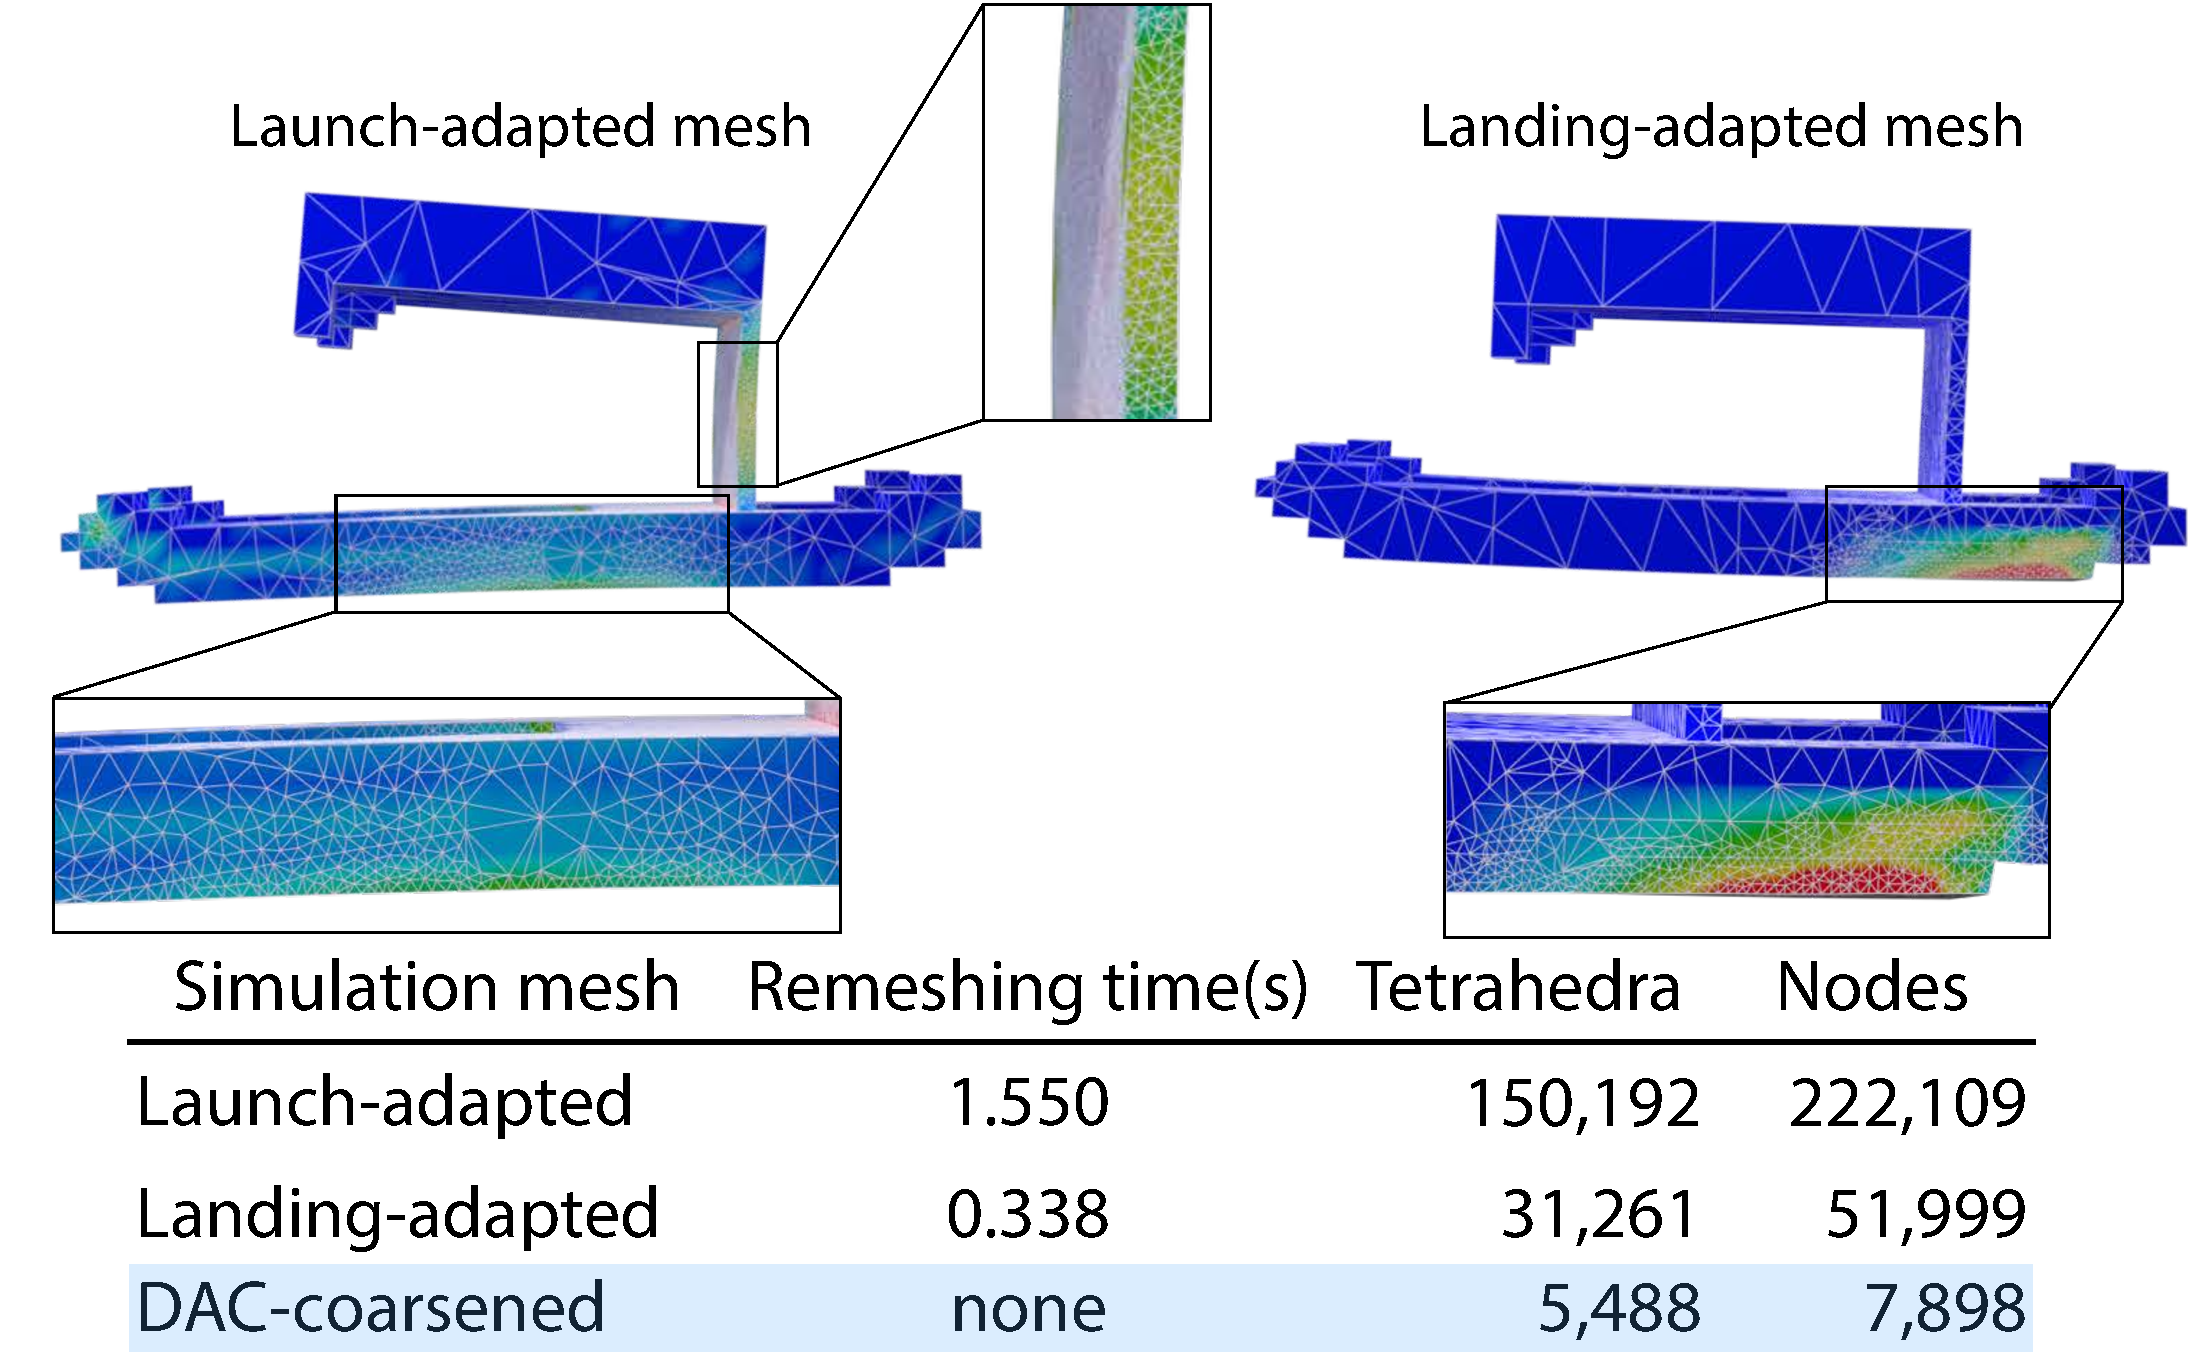
\includegraphics[width=0.7\columnwidth]{./figs/Adaptive_Meshing}	
	\caption{Comparing adaptivity and coarsening. A tetrahedral model of a jumper is adaptively remeshed to capture input stress fields from its launch and landing states. We compare the resulting element and node counts to our DAC-coarsened model. We set the minimum edge length for remeshing to one that was experimentally found to yield convergent numerical results.}
	\label{fig:adaptiveMeshing}
\end{figure}

\emph{Adaptive meshing} allows us to reduce element counts in material regions where refinement is less critical.
Let us ignore the difficulty of implementing adaptive meshing and the per time step cost to remesh. Even so, adaptive meshes are challenging in our setting. We model objects that undergo rapidly changing boundary conditions and globally varying stress fields due to contacts, loading and impacts. Adaptive meshing in our setting must then, necessarily, feature high numbers of elements to capture these details. See Figure~\ref{fig:adaptiveMeshing}. Here, using our experimentally validated, accurate element edge length as adaptive meshing threshold, our tetrahedral mesh contains 6.5X to 28X more nodal DoFs than our corresponding DAC-coarsened mesh. The DAC-coarsened mesh is likewise simpler to implement and has no per time step computational cost. 

\emph{Reduced models} utilizing linear modes~\cite{James:2002:DDR,Hauser:2003:IDU} are widely applied to accelerate dynamic simulations. The key issue here is that linear modal models provide only a \emph{linear} approximation of the deformation space leading to inaccurate linearization artifacts, 
such as swelling during rotation;
see Figure~\ref{fig:modalModels}. Optimized quadrature approaches, in turn, can afford efficient integration of non-linear forcing functions, but do not alleviate these artifacts~\cite{An:2008:OCE} when relying on an underlying modal deformation space.
Finally, nonlinear modal models~\cite{Barbic:subspace:2005} can alleviate some of these issues but so-far remain challenging to incorporate in the design process in comparison to their linear counterparts~\cite{Chinesta2013}. 

\begin{figure}
	\centering
	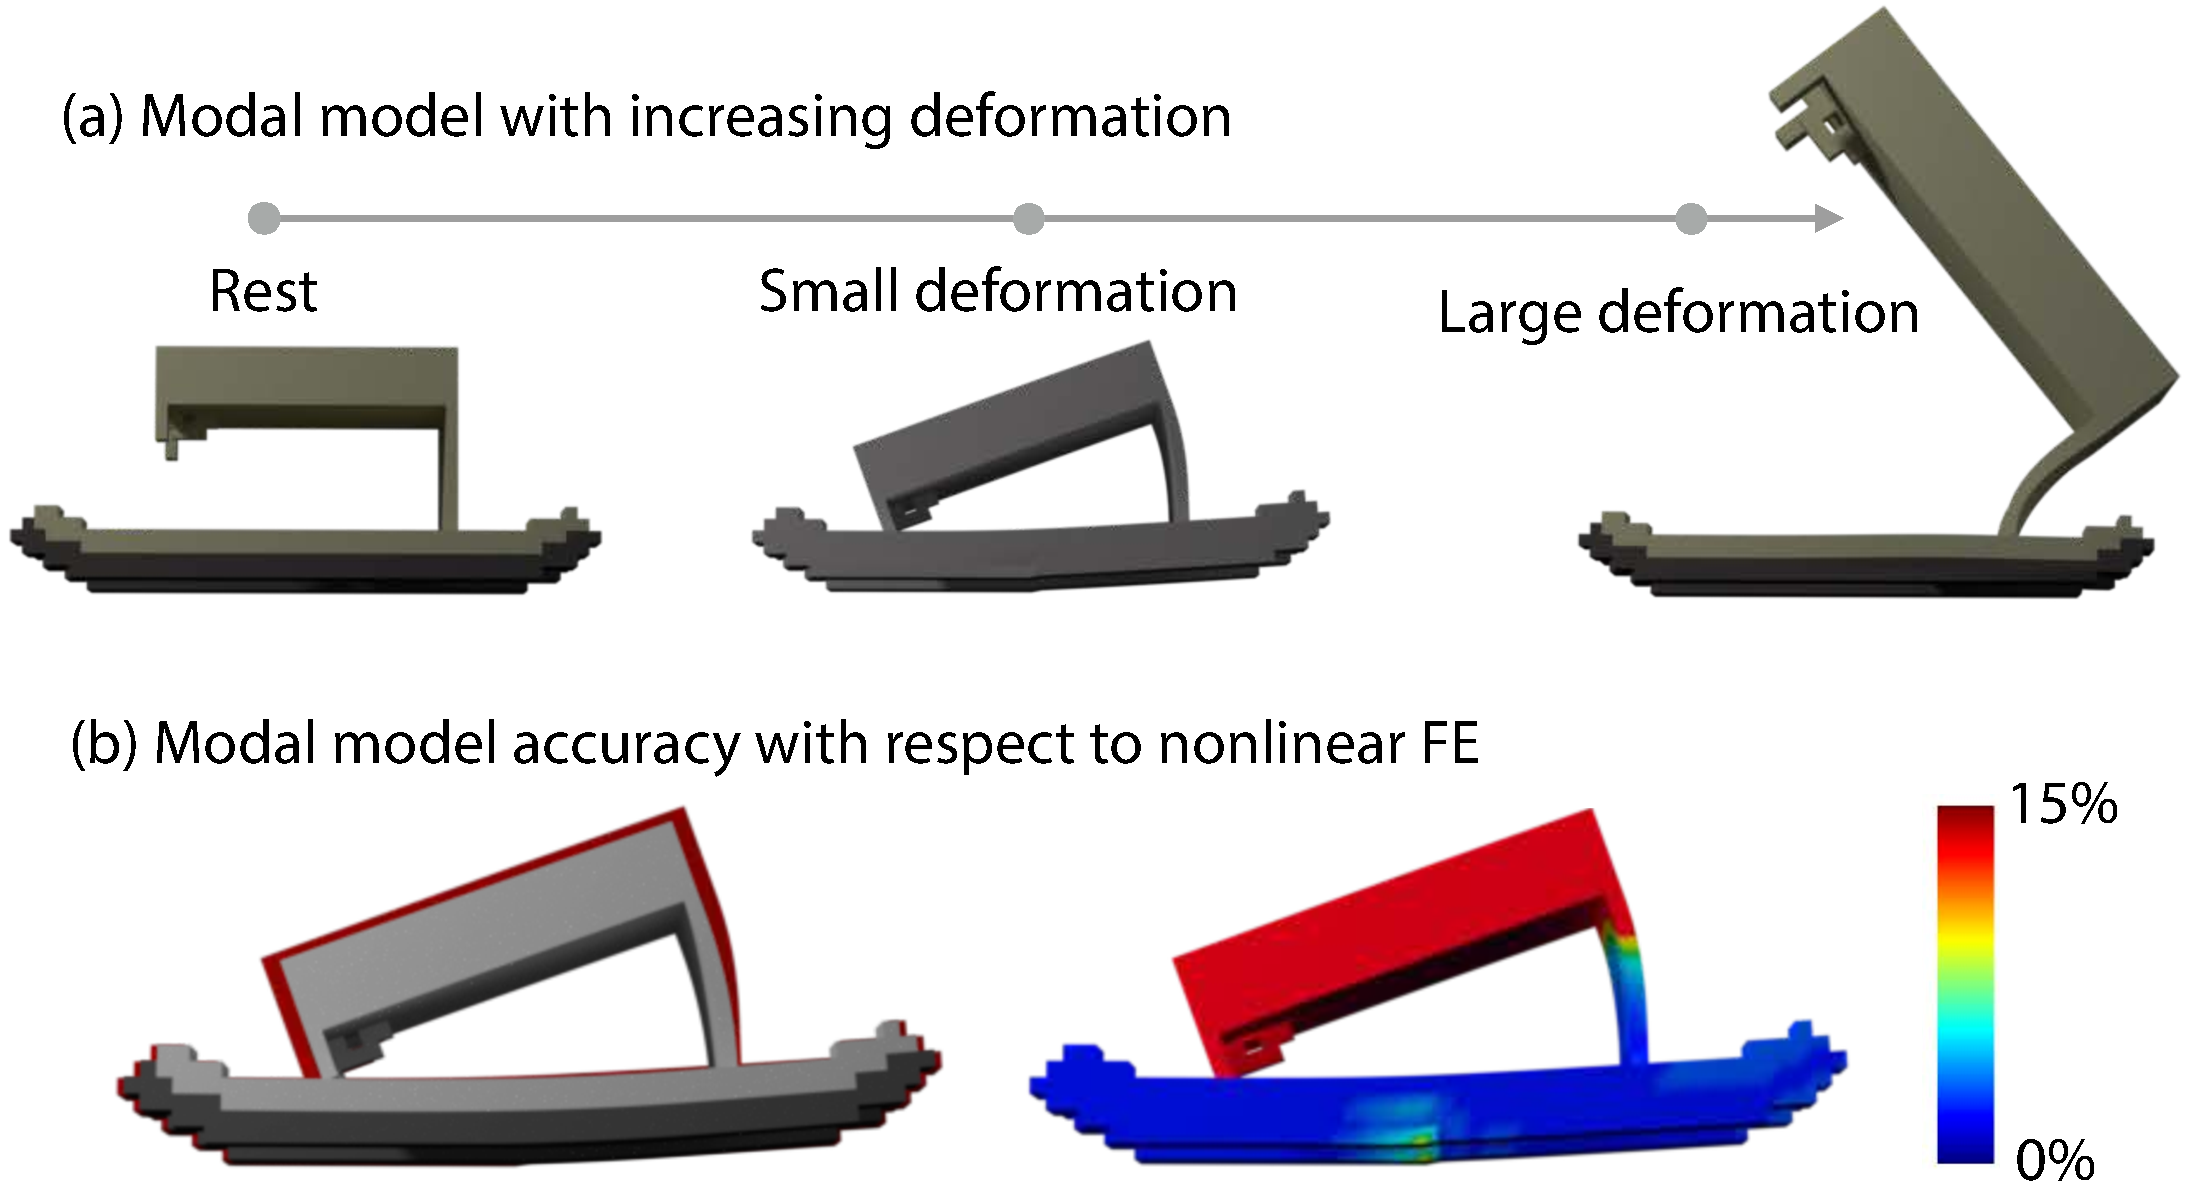
\includegraphics[width=\columnwidth]{figs/Modal_Expansion}
	\caption{Linear modal models suffer from distortion as deformations grow. In (a) we illustrate increasing deformations, left to right, with corresponding inflation errors. Even for smaller deformations, (a) middle, the linear modal model still introduces significant distortions leading to modeling inaccuracies. In (b), left, we overlay simulations of small deformation  performed respectively with the linear modal model (red) and the coarsened nonlinear FE model (grey); and, on the right, evaluate accuracy of the modal model. During simulation, even these smaller deformations introduce inaccuracies in the modal model due to element inflation; here up to 13.7\%.} 
	\label{fig:modalModels}	
\end{figure}

We begin by observing that \emph{numerical coarsening} offers an exciting alternative for efficient yet predictive FE modeling. Coarsening methods effectively apply coarse resolution FE meshes as reduced DoF models and then seek material models that reproduce the behavior of a high-resolution FE counterpart. Analytical solutions for coarsening have been developed for linear material models (models where the stress varies linearly with strain)~\cite{Kharevych:2009cg,Nesme:2009:PTE,Torres:2016:HIC}.
Due to this linear assumption, and similarly to the linear modal models discussed above, we find them difficult to apply for the accurate modeling of the nonlinear materials required for 3D-printed objects.
Even more recently, data-driven coarsening strategies~\cite{chen2015:ddfem} have been proposed to overcome the linear limitation of prior work. Unfortunately, while coarsening offers promise, prior work, to our knowledge, does not account dynamic effects, inertial properties, nor material damping characteristics.
As we see in Figure~\ref{fig:coarse}, this causes even the most recent, nonlinear, data-driven coarsening approaches to produce highly inaccurate dynamic simulations.

Building on the promise of coarsening techniques and inspired by recent developments in frequency matching for plausible computer animation~\cite{Li:2014:SEE,BinWang:2015fx}, we develop a new, dynamics-aware coarsening (DAC) method that, in contrast to prior approaches, provides well-over an order-of-magnitude performance enhancement, while maintaining fabrication-level accuracy when modeling highly dynamic motions subject to frictional contact. Our method does so without complex substructuring, does not require adaptive remeshing, accounts for dynamic effects including damping, and does not introduce prohibitive linear modeling artifacts and so is applicable to a wide selection of nonlinear constitutive models for 3D-printed materials.  

\subsection{Impact Response for Elastic Materials}
Even with a suitably accurate FE solution to model \emph{material} dynamics, accurate impact response for elastic materials on collision remains highly challenging.  To capture the bounces and rebounds of elastic mechanisms coming into contact with the ground - consider for example the heel strike of a sneaker - we need to get this right. State-of-the-art, implicit time-stepping methods for FEM with contact solve variational forms of time-steppers, e.g., variational Implicit Newmark, subject to additional, fully implicit contact and friction forces~\cite{Kane:1999kr,Pandolfi:2002ik}. 
These form so-called nonsmooth or \emph{complementarity} integrators. 


\begin{figure}
	\centering
	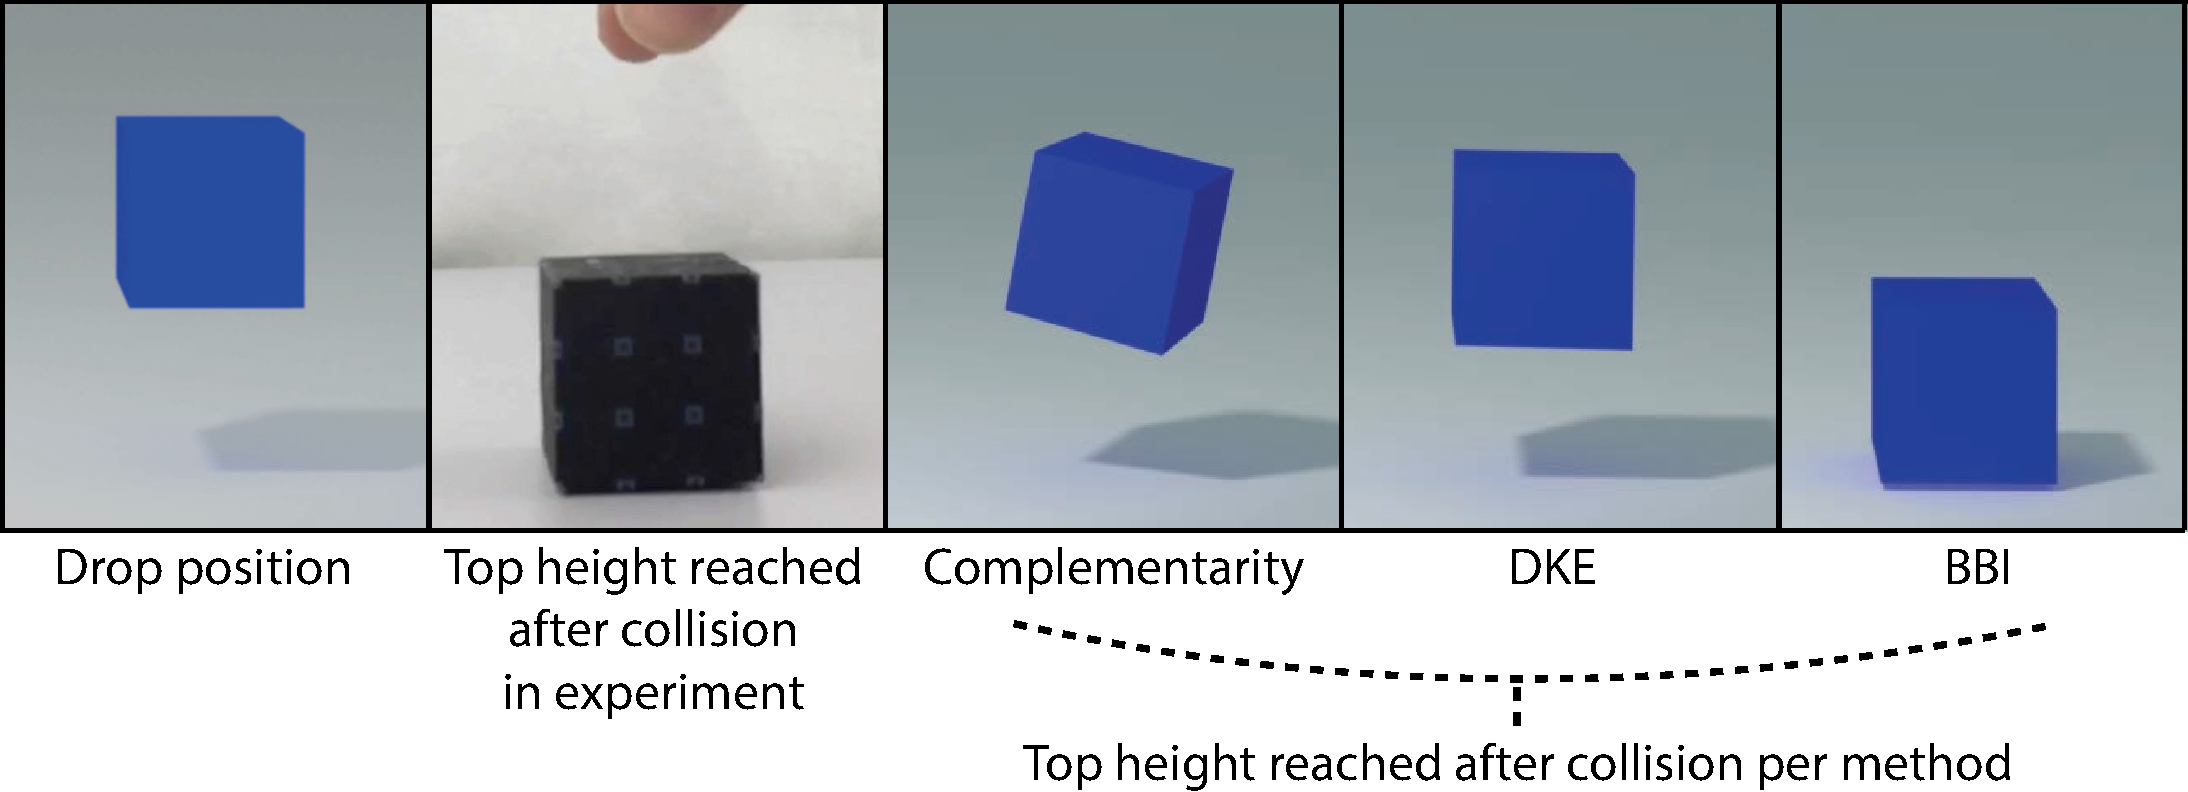
\includegraphics[width=\columnwidth]{figs/Figure_2_BBI}	
	\caption{Comparison of complementarity Newmark integration, DKE Stabilization and our BBI model for the impact resolution of an elastic, 3D-printed block. BBI closely matches the maximum rebound height achieved by the experimental result while both the Complementarity and DKE methods overestimate the rebound significantly.}
	\label{fig:BBI_block_compare}
\end{figure}

However, these complementarity integrators have two well-known flaws~\cite{Deuflhard:2008fu}: (1) these methods can yield spurious oscillations on the contact boundaries and (2) the effective impact response of these methods is too energetic. Effectively the normal velocity on impact along the elastic boundary should be dissipated completely. Instead, complementarity methods with Newmark will generate an entirely incorrect elastic restitution; see Figure~\ref{fig:BBI_block_compare}. To address these problems~\citet{Deuflhard:2008fu} introduced the now-standard DKE contact-stabilization step to filter contact response with projection. In the limit, DKE makes the impact-response model consistent,
while in FE codes it is applied as an effective strategy to recover from the well-known limitations of implicit integration with impact. However, it remains widely acknowledged that the right-way to accurately model high-speed collision response with implicit FE remains an open question at this time - not only in graphics - but more broadly in scientific computing as well. As an example consider Figure~\ref{fig:BBI_block_compare} where we see that both the complementarity model \emph{and} the DKE filter produce different but equally incorrect predictions of the response of a stiff elastic block dropped on the floor. Here we offer a new, Boundary-Balancing Impact (BBI) model for FE that gains us accurate prediction of impact response for the stiff 3D-printed materials we focus on here; see Figure~\ref{fig:BBI_block_compare}.

\subsection{Summary}
High-fidelity simulation methods for elastodynamics are too slow for use in fabrication design tasks while existing strategies to reduce the simulation cost of elastica (including adaptive, reduced and coarsened models) are too inaccurate and/or too expensive to employ. Finally, existing FE models for simulating elastic collision and rebound miss critical compliance coupling in the filter stage.

\subsection{Contributions}
We have exposed and analyzed the limitations of simulation methods for the predictive modeling of elastodynamics at rates sufficient for fabrication design optimization. Next, we develop our \emph{Dynamics-Aware Coarsening} (DAC) method to address this need {(\S3)}. DAC jointly identifies \emph{and} predictively simulates fabricated materials. To address current limitations in FE collision-response filtering we then introduce our \emph{Boundary Balancing Impact} (BBI) model {(\S4)}. 
We then validate these contributions by comparing simulated results generated by DAC and BBI with real-world results experimentally obtained from a range of compliant 3D-printed jumping and throwing mechanisms that flip, throw projectiles, jump onto obstacles and jump over walls (\S5).